% ===================================================
% CHAPITRE 18 — VICAIRES D'OUROUX
% Pages imprimées 167-175 — vues 170-178
% ===================================================
\chapter{Vicaires d'Ouroux}

% --- Page imprimée 167 — vue 170
\ourouxlettrine{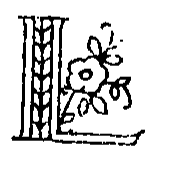
\includegraphics[height=4\baselineskip]{Illustrations/lettrines/lettrine-l.png}}{e vicariat d'Ouroux n'a pas toujours existé ; il a subi pendant les deux derniers siècles de fréquentes vicissitudes, soit par suite du manque de ressources, soit à cause du petit nombre de prêtres qui étaient à la disposition des évêques. Je passe sous silence la longue période pendant laquelle la paroisse d'Ouroux fut desservie par des prêtres sociétaires qui portaient le titre de vicaires perpétuels. Ils étaient, à vrai dire, de véritables curés et ils en exerçaient les charges.}

Le premier vicaire qui nous est connu est :

1 - \underline{Pierre Mollaret} présent au dénombrement des habitants de la paroisse d'Ouroux fait à l'occasion d'un procès intenté par Mr Morin, curé, contre MM. les Doyens Chanoines et Chapitre Notre-Dame de Beaujeu qui ont usurpé une partie des revenus de la cure. L'acte est du 13 février 1667.

% --- Page imprimée 168 — vue 171
II-\underline{Jean Fretière} que nous trouvons à Ouroux comme vicaire le 13 Janvier 1676, puis curé de St-Christophe-la-Montagne en 1682.

III-\underline{N. Rochard} administre la paroisse de concert avec Mr de Grosbois du 17 Décembre 1732 au 25 Septembre 1733 pendant la vacance de la cure, à la suite du départ de Mr Perrachon. À quel titre était-il à Ouroux ? On ne peut formuler à ce sujet que des conjectures. Il n'a jamais eu le titre de curé, mais celui de vicaire. Et cependant à cette époque le vicariat n'existait pas comme nous le verrons plus bas. Mr Perrachon, à son départ, conservant son titre de curé confia-t-il l'administration de la paroisse à Mr Rochard ou bien Mr Guillin ayant été investi du bénéfice, le chargea-t-il de sa direction en attendant qu'il eût terminé ses études, comme cela avait lieu fréquemment ? Les deux hypothèses sont possibles.

IV-\underline{Étienne Buffin} fut autorisé à exercer les fonctions de vicaire par Mr Gabriel François Moreau évêque de Mâcon le 20 Août 1766. Le Chapitre de Beaujeu néanmoins qui était décimateur dans la paroisse ne lui donnait aucune part sur les revenus du bénéfice. Mr Guillin adressa alors une requête à Monseigneur donnant pour motifs l'étendue considérable de la paroisse et l'augmentation du nombre des communiants depuis la dernière visite de l'évêque de Mâcon qui avait eu lieu en 1746.

Sa requête fut agréée et communiquée au Chapitre de Beaujeu. Mr Guillin la leur fit signifier ensuite par huissier. Mr Brac de Chasté, chanoine, lui répondit le même jour qu'il serait libre à Mr Guillin de prendre sur les revenus du chapitre l'honoraire nécessaire, pour l'entretien du vicaire. À cette époque (1768) cet honoraire était évalué à 200 livres ; en 1778 il fut porté à 250 et enfin en 1785 à 350 livres.

Monseigneur confirma donc la nomination de Mr Buffin ; l'acte authentique est conservé dans les archives de la paroisse ; il est daté du 14 Septembre 1767.

Le dernier acte signé par Mr Buffin est du 17 Octobre 1767 ; il eut pour successeur :

% --- Page imprimée 169 — vue 172
V-\underline{François Trouilloux} qui devait un jour remplacer Mr Guillin comme curé. Nommé le 2 Novembre 1768 il desservit la paroisse pendant près de dix ans, c'est-à-dire jusqu'au 8 février 1768, date de la mort de Mr Guillin.

Après lui, le vicariat d'Ouroux vit passer un nombre relativement considérable de prêtres qui se succédèrent avec une fréquence étonnante. A peine leurs noms nous ont-ils été conservés par les registres de catholicité.

VI-\underline{N.. Puy} succéda à Mr Trouilloux en Mars 1778. Il n'était plus à Ouroux au mois de Novembre de la même année. Il fut remplacé par :

VII-\underline{N.. Barnaud} qui vint en Novembre 1778 et desservit la paroisse jusqu'en novembre 1779. Deux ans après fut nommé :

VIII-\underline{N.. Callier} qui vint en Septembre 1780 et partit au bout de quelques mois. Nouvel intervalle de plus de trois ans, jusqu'à

IX-\underline{N.. Arthaud} qui fut nommé le 22 Février 1784 et repartit au mois de Novembre de la même année. Vint ensuite :

X-\underline{N.. Thibert} qui n'occupa le poste que jusqu'au 20 Mai 1785

XI-\underline{N.. Mouche} n'a mis sa signature qu'au bas de deux actes. Il est probable que Mr Trouilloux demeura seul jusqu'au mois de Juin 1788, époque à laquelle fut nommé :

XII-\underline{Antoine Odin} avec lequel il ne devait encore demeurer que peu de temps. Mais étrange contraste ! Cette fois ce fut Mr Trouilloux qui partit et le vicaire eut la gloire de demeurer ferme à son poste.

Après le Concordat et le départ de Mr Odin à St-Nizier-d'Azergues Mr Trouilloux n'eut pas de vicaire. Les prêtres décimés par la Révolution étaient, on le comprend, fort peu nombreux. Ouroux ne pouvait donc pas espérer de voir rétablir le vicariat dans la nouvelle organisation des paroisses. Pendant 13 ans Mr Trouilloux fut obligé de desservir seul la paroisse, malgré son âge et ses infirmités.

{\setlength{\emergencystretch}{2em}
L'administration épiscopale, néanmoins, ayant regard aux services rendus par le vénérable vieillard, connaissant d'ailleurs l'impossibilité
% --- Page imprimée 170 — vue 173 (suite)
dans laquelle il était de faire le bien par suite de sa cécité, accéda enfin à sa demande et nomma comme vicaire, au mois d'Août, 1813 :\par}

XIII - \underline{N. Duvernay} qui séjourna à Ouroux jusqu'au 1er Octobre 1814

XIV - \underline{Pierre Marie Polloce} ne succéda pas à ce dernier immédiatement. Il fut nommé le 28 Août 1815. Il devait bientôt succéder à Mr Trouilloux comme celui-ci avait succédé à Mr Guillin.

Mr Polloce était jeune, actif. En prenant la succession de son vénéré curé, il était naturel qu'il fût chargé seul de l'administration de la paroisse. Mais enfin il dut demander à son tour un collaborateur.

XV - \underline{Morétain} fut nommé vicaire d'Ouroux le 5 Juin 1844. À cette époque le vicariat n'était pas reconnu et malgré les démarches souvent renouvelées de Mr Polloce et du Conseil de Fabrique il ne fut reconnu par le gouvernement qu'en 1848.

\enlargethispage{2\baselineskip}
Je n'ai pas à retracer ici cette vie qui sera une des gloires de notre paroisse et qui a fait l'objet d'un travail spécial. Il suffira de rappeler que Mr Morétain seconda dignement celui que la Providence lui avait donné pour père. Dans les moments difficiles qu'ils eurent à traverser ensemble, Mr Polloce trouva dans son auxiliaire cette énergie persévérante et tenace qui le distingua plus particulièrement pendant tout son ministère.

C'est à Mr Morétain que nous devons les chapiteaux qui ornent les colonnes de l'église et le tabernacle du maître-autel.

Se sentant appelé à un apostolat plus difficile mais aussi plus fructueux que celui qu'il exerçait à Ouroux, il résolut de se consacrer aux missions de Palestine. Mr Poyet, prêtre Lyonnais, était précisément venu en France pour trouver quelques prêtres qui voulussent se dévouer à cette œuvre.

Mr Morétain quitta Ouroux en 1852. Il débuta dans l'île de Chypre où il séjourna néanmoins quelques mois. L'année suivante il fut appelé par le Patriarche de Jérusalem, Mgr Laverga, pour fonder la première mission de la Palestine à Beit-Djalla, gros bourg de trois mille habitants, situé à deux kilomètres de Bethléem.

% --- Page imprimée 171 — vue 174
L'entreprise était difficile ; deux fois les Pères Franciscains de Terre Sainte avaient dû renoncer. Mgr Valerga le savait et cependant il fallait réussir à tout prix ; l'avenir des missions à fonder en dépendait absolument. Aussi s'assura-t-il de la protection française par une déclaration nette, explicite tant de la part du ministère que de l'ambassade de Constantinople.

Pour ne pas éveiller les susceptibilités des schismatiques grecs Mr Morétain partit seul, avec un domestique fidèle et un chameau portant les effets de première nécessité. Mais la population avait été prévenue ; les habitants coururent aux armes et défendirent l'entrée de leur bourgade au missionnaire qui fut contraint de se retirer à Bethléem. Quelques jours après, une escouade de soldats l'introduisait dans le village récalcitrant et le mettait en possession de la maison achetée par le Patriarche.

Les grecs irrités résolurent de chasser à tout prix Mr Morétain. Le Patriarche informé de leurs projets accourut à Beit-Djalla défendre lui-même son missionnaire. La lutte fut longue. Mr Lequeux, chancelier du Consulat de Jérusalem, informé de ce qui se passait, vint à son tour encourager à la résistance. Ni menaces, ni promesses ne peuvent émouvoir les ennemis du catholicisme. Le 9 Décembre, après un siège de trois heures, ils parviennent à enfoncer la porte de la demeure du missionnaire, exigent que Mgr Valerga parte et consentent à laisser Mr Morétain dans sa demeure jusqu'à l'envoyé du Pacha que l'on attendait impatiemment.

Le Patriarche profita du silence de la nuit pour gagner à sa cause le Musulman qui était à la tête de ses ennemis ; six cents piastres eurent raison de ses scrupules : Les cavaliers envoyés de Jérusalem et qui n'avaient osé s'interposer au milieu de la lutte, gagnés à leur tour, firent évacuer de vive force la maison, le 10 décembre au matin. L'un des insurgés, furieux de l'échec que son parti vient de subir, sachant que Mr Morétain est à l'autel, tire un coup de fusil par la fenêtre dans l'intention évidente de le tuer. La balle traverse le volet, frappe la voûte de la chambre, passe par ricochet au-dessus de sa tête et vient tomber à ses pieds. Mr Morétain admirable
% --- Page imprimée 172 — vue 175 (suite)
de sang froid, la ramasse, la met sur l'autel aux pieds du crucifix remerciant Marie d'une protection aussi visible.

Malgré un firman favorable au Patriarche, les conjurés ne désarmèrent pas ; mais ils durent remettre à une époque ultérieure l'attaque projetée, le pacha ayant consenti à donner au Patriarche quelques soldats. Elle eut lieu le 6 Février et cette fois-ci encore la vie de Mr Morétain fut sérieusement en danger. Le consul comprit qu'il fallait enfin en finir. Il déclara au Divan que si les coupables n'étaient pas arrêtés et punis, il quittait Jérusalem ainsi que Mgr Valerga.

Satisfaction ne leur ayant pas été accordée, le Consul, Paul Émile Botta, Mr Lequeux, le Patriarche, Mr Morétain et leur suite escortée de quinze cavaliers prirent la route de Jaffa où ils séjournèrent pendant six mois. Le gouvernement français mit beaucoup de bonne volonté dans ses réclamations et obtint de la Sublime-Porte un firman solennel ordonnant au Patriarche grec de Jérusalem de ramener le Patriarche latin à Jérusalem, puis à Beit-Djalla et de lui assurer, aux frais du gouvernement l'achat du terroir nécessaire pour bâtir une église et une maison pour son missionnaire.

Le triomphe était complet. Rentré dans sa mission, Mr Morétain se mit aussitôt à l'œuvre. Il fit construire des écoles, un presbytère, une église gothique et le séminaire.

À peine ces constructions étaient-elles terminées que le Patriarche l'appela à fonder une nouvelle mission, celle de Beit-Schour, ou village des Pasteurs. Il y arriva le jour de Noël de l'année 1859 Il acheta immédiatement le terrain nécessaire à la construction de la chapelle, des écoles, de la maison des missionnaires et du cimetière. Pour les ressources exigées par ces divers travaux, il s'adressa plus spécialement aux catholiques de Pologne.

À peine cette mission était-elle fondée que Mr Morétain fut appelé par le Patriarche à en établir une nouvelle au Salt, gros bourg situé de l'autre côté du Jourdain. Là encore tout était à faire ; il commença la construction de l'église qu'il dut interrompre faute de ressources. Mgr, lui ayant donné un vicaire, il revint à Beit Sahour dont il était resté le titulaire.

% --- Page imprimée 173 — vue 176
Enfin Monsieur Morétain, réduit par ses infirmités à une impossibilité absolue de travailler, quitte Beit-Sahour le 4 Décembre 1878 pour se retirer au patriarcat. Là, pendant cinq ans, il édifia ses frères dans le sacerdoce par son esprit de foi et son courage au milieu des souffrances qu'il avait à supporter. Il mourut le 13 Avril 1883.

{\setlength{\emergencystretch}{2em}
XVI-\underline{Jean Marcellin Alvergnat} né à Rozier-Côte d'Aurec, canton de St-Bonnet le Château (Loire) fut installé vicaire à Ouroux le 16 Novembre 1852. Il est décédé curé à Lafont, paroisse fondée vers la fin du XIXe siècle, dans l'archiprêtré de St-Nisier d'Azergues. Il eut pour successeur :\par}

XVII-\underline{Jean Antoine Marie Dubessy} né à St Forgeux, installé à Ouroux le 29 Novembre 1862. Il devint ensuite curé de St-Christophe-la-Montagne.

XVIII-\underline{Antoine Chapelon} né au Chambon Feugerolles (Loirs) lui succéda le 25 Juin 1871. Il fut nommé au mois d'Octobre 1878 vicaire à Ste-Marie à St-Étienne (Loire) et en 1899 curé de St-Marcellin (Loire)

XIX-\underline{Alexandre Peronnet} ne séjourna à Ouroux que quelques mois, du 20 Octobre 1878 au mois de Juin de l'année suivante, époque où il fut nommé vicaire à Condrieu

\noindent\hbox to \textwidth{\leaders\hbox to 0.45em{\hss-\hss}\hfill}\par
\begin{tabbing}
\hspace{0.10\textwidth}\=\kill
\>Ici s'arrête la liste des vicaires dressée par l'Abbé Odouard,\\
\>Voici quels furent les derniers vicaires d'Ouroux.
\end{tabbing}
\noindent\hbox to \textwidth{\leaders\hbox to 0.45em{\hss-\hss}\hfill}\par

XX-\underline{Germain Odouard} fut installé comme vicaire à Ouroux le 20 Juin 1879. Il quitta Ouroux en l'année 1892 et il devint successivement curé de Trades, de St-Bonnet-les-Bruyères et de Monsols. Il mourut au mois de Septembre 1929.

L'Abbé Odouard se plaisait à étudier l'histoire locale. Comme il a été dit dans la Préface de ce livre, il fit œuvre de véritable historien. Durant son vicariat, il écrivit l'Histoire d'Ouroux, puis une Vie de l'Abbé Morétain. Curé, il écrivit l'Histoire de Monsols, de St-Rigaud, etc.

% --- Page imprimée 174 — vue 177
L'Abbé Odouard fut l'un des vicaires d'Ouroux dont les anciens qui l'ont connu ont gardé un excellent souvenir. Il était très alerte, actif et dévoué. Il avait toujours quelques bons mots à dire, avait réponse à tout, était aimé des enfants. À plus d'un, au cours de ses visites, il donnait quelques conseils, voire même quelques recettes pratiques d'ordre matériel. Un des anciens de la paroisse nous racontait, lors d'une réunion à la cure, faite en septembre 1952 pour rassembler tous les vieux souvenirs de mémoire d'homme, qu'étant petit berger il se trouvait dans un pré du côté de "Rateau". L'abbé Odouard, de passage en cet endroit, lui avait appris la façon de calculer la hauteur d'un peuplier en mesurant son ombre avec la longueur de l'ombre d'un bâton enfoncé en terre et mesurant un mètre au-dessus du sol.

L'abbé Odouard avait beaucoup de talent. Sa connaissance de la musique lui permit de former une belle chorale. À son départ d'Ouroux il fut remplacé par l'Abbé :

XXI-\underline{Antoine Magnin} qui arriva à Ouroux le 20 Juin 1892. Comme son prédécesseur, l'Abbé Magnin était très bon musicien et la chorale d'Ouroux connut avec lui une époque très florissante. Parmi les chantres beaucoup étaient des hommes mariés qui continuaient à faire partie de la chorale. Ce qui facilitait les répétitions de chant c'est qu'un certain nombre, ayant fréquenté le pensionnat des frères à Beaujeu, connaissait le solfège. De l'abbé Magnin on a gardé le souvenir aussi d'un prédicateur qui faisait de longs sermons. Il fut ensuite nommé vicaire à St-Étienne (Loire) puis curé des Sauvages (Rhône).

XXII-\underline{Joseph Grollier} arrivait à Ouroux le 26 Septembre 1897. À peine deux ans après son arrivée il partait comme vicaire à Fleurie. Il fut remplacé par :

XXIII-\underline{Jean Louison} arrivé le 3 juin 1899 qui resta seulement un an à Ouroux et partit comme vicaire à Montaud à St-Étienne.

XXIV-\underline{Mathieu Deschavanne} vicaire dans notre paroisse à partir du 24 Juin 1900 resta deux ans parmi nous. Il fut nommé ensuite vicaire
% --- Page imprimée 175 — vue 178 (suite)
à Chambost-Longessaigne, puis au Sacré-Cœur à Lyon.

XXV-\underline{Eugène Valarin} nommé à Ouroux, arriva le 25 Mai 1902. Il fut ensuite vicaire à Montagny (Loire).

XXVI-\underline{Jean Daviet} fut vicaire à Ouroux. Il arriva le 14 novembre 1903. Il devint ensuite aumônier de l'orphelinat de St-Sorlin (Rhône).

XXVII-\underline{Jean Grapeloup}, prêtre du Prado arriva à Ouroux le 18 juin 1905. Il fut ensuite vicaire à Lyon, puis curé à St-Joseph. Actuellement, (en 1952) il est aumônier à l'hôpital St-Luc à Lyon.

XXVIII-\underline{Joseph Marcel} fut vicaire pendant 4 ans à Ouroux, du 15 janvier 1908 en décembre 1912. Il s'occupait beaucoup du patronage des enfants ainsi que des répétitions de plain-chant. Il quitte Ouroux pour aller vicaire à Villars.

XXIX-\underline{Claude Clément} arriva à Ouroux le 24 décembre 1912. Il était né à Chenelette (14 mars 1886) mais ses parents habitèrent ensuite sur la paroisse des Ardillats.

L'abbé Clément remplit son ministère de vicaire dans notre paroisse jusqu'à la guerre de 1914--1918. Mobilisé il fut un des premiers à partir d'Ouroux. Il mourut sur le champ de bataille, pour la France, tué par une balle allemande, à Tracy-le-Val, le 24 novembre 1914.

Durant son vicariat l'Abbé Clément s'occupa beaucoup de l'apostolat eucharistique. Suivant en cela les directives du Pape Pie X et rompant avec les usages récents, il rappela que les petits enfants, dès l'âge de raison, peuvent s'approcher de la sainte table. Il prêcha aussi la Communion fréquente.

L'Abbé Clément fut le dernier vicaire d'Ouroux.
